\documentclass[conference,a4paper]{IEEEtran}
% ICCIT 2026 uses double-blind review. Add author details only for the camera-ready paper.

\usepackage{cite}
\usepackage{amsmath,amssymb,amsfonts}
\usepackage{graphicx}
\usepackage{textcomp}
\usepackage{xcolor}
\usepackage{booktabs}
\usepackage{tabularx}
\usepackage{array}
\usepackage{tikz}
\usepackage{url}
\usetikzlibrary{arrows.meta,calc,fit,positioning,decorations.pathreplacing}
\urlstyle{same}

\definecolor{jbblue}{RGB}{35,91,133}
\definecolor{jbteal}{RGB}{35,116,105}
\definecolor{jbamber}{RGB}{171,106,29}
\definecolor{jbred}{RGB}{158,48,48}
\definecolor{jbgray}{RGB}{241,243,245}
\definecolor{jbink}{RGB}{39,50,56}

\def\BibTeX{{\rm B\kern-.05em{\sc i\kern-.025em b}\kern-.08em
    T\kern-.1667em\lower.7ex\hbox{E}\kern-.125emX}}

\begin{document}

\title{Partition-Tolerant Federation Across Simulated ISP Islands}

\author{Anonymous submission}

\maketitle

\begin{abstract}
An Internet shutdown may remove international routes while leaving small groups of domestic
networks connected. We study whether federated forum servers can continue to accept and exchange
public posts over those remaining paths. The prototype uses canonical protobuf envelopes, author
signatures, signed acceptance receipts, caller-initiated synchronization, and a trusted dual-homed
server that can relay between isolated network groups. In a four-node Docker testbed, after the
ordinary route between two groups was removed, a certificate, community, and post reached the other
group in 0.5, 1.2, and 2.1 seconds. In a separate eight-node in-process chain, all 200 envelopes
reached the seventh hop, with a median of 4.125 seconds and a 99th percentile of 6.115 seconds.
TypeScript, Rust, and Python implementations agreed on all 16 test vectors. A malformed-input run
created no invalid storage writes, although most requests were stopped by rate limiting. The signed
protobuf representation used 4.4 to 6.9 times fewer bytes than gzipped ActivityPub JSON-LD in the
measured sample. This compact format gives up ActivityPub interoperability, mature tools, and
flexible JSON-LD extensions. The results show that the mechanism works in a controlled single-host
test when some IP paths survive. They do not show operation during a total blackout, across real
Internet service providers, or under a strong denial-of-service attack.
\end{abstract}

\begin{IEEEkeywords}
federated systems, Internet shutdowns, network partitions, signed objects, store-and-forward
\end{IEEEkeywords}

\section{Introduction}

Internet shutdowns are not always a single on-or-off event. A disruption may involve throttling,
destination blocking, protocol filtering, or the loss of international routes
\cite{bischof2023shutdowns,ooni2025bangladesh}. Some networks may still reach each other while other
networks are cut off. Baltra \emph{et al.} call these reachable groups \emph{connectivity islands}
\cite{baltra2024connectivity}. This paper asks a narrow question: if some domestic Internet Protocol
(IP) paths remain, can independent forum servers continue to accept signed posts and synchronize
them across the remaining network graph?

Existing systems solve related but different problems. Circumvention systems connect a user to an
external service through cooperating infrastructure or temporary proxies
\cite{wustrow2011telex,bocovich2024snowflake}. Phone-to-phone systems use Bluetooth or Wi-Fi Direct
when packet networks are absent \cite{kamali2025anix,lerner2016rangzen,pradeep2022moby}. These
systems are important during a full blackout, but they do not define how independently operated
domestic servers should validate, store, and relay public forum objects when only partial IP
connectivity remains.

We present a server-federated design for this condition. An author signs one exact byte sequence.
Every receiving server checks the same bytes, stores them with a content identifier, and returns a
signed receipt after acceptance. A server can start delivery, streaming, or backfill even if it
cannot accept inbound connections. If two islands cannot reach each other directly, an explicitly
trusted dual-homed server can validate, store, and relay objects between them.

The paper makes four contributions:

\begin{itemize}
  \item a byte-preserving admission path for both local and federated signed objects;
  \item caller-initiated delivery and recovery for asymmetric network reachability;
  \item a rate-limited bridge policy that validates every object and avoids relay loops; and
  \item controlled evidence from cross-language vectors, a Docker route-cut test, an eight-node
        chain, a malformed-input run, and a measured ActivityPub encoding comparison.
\end{itemize}

The claim is limited to \emph{partition tolerance under surviving IP paths}. The system cannot
create a route during a total communication blackout, hide a visible bridge from a network
operator, or force an operator to accept a valid post.

\section{Background and Research Gap}
\label{sec:background}

\textbf{Federated and signed systems:} ActivityPub sends social activities to server inboxes
\cite{activitypub}. Matrix and AT Protocol also support server federation or repository replication
\cite{matrixspec,atproto}. Nostr and Secure Scuttlebutt replicate signed content
\cite{nostr,tarr2019ssb}. These systems provide useful building blocks, but normally reachable
server addresses remain important. They do not combine exact-byte admission, operator receipts,
outbound-only recovery, and an explicit two-island relay policy in the form evaluated here.

\textbf{Blackout communication:} Anix, Rangzen, Moby, and Twimight exchange data through nearby
devices \cite{kamali2025anix,lerner2016rangzen,pradeep2022moby,hossmann2011twimight}. Dolphin uses a
cellular voice channel when packet data is blocked \cite{sharma2023dolphin}. These designs give up
some latency, bandwidth, or battery life so that they can work without a domestic server path. Our
design makes the opposite trade-off. It can be faster while servers remain connected, but it stops
cross-island delivery when all IP paths disappear.

\textbf{Accountability:} Certificate Transparency uses append-only logs, signed tree heads, and
proofs to make some forms of misbehavior visible \cite{rfc6962,rfc9162}. PeerReview and CoSi study
stronger distributed accountability \cite{haeberlen2007peerreview,syta2016cosi}. A receipt in our
system proves that one operator acknowledged one object. It does not prove that the operator accepts
all valid objects or forwards them on time.

The research gap sits between normally routed federation and device-to-device blackout networks.
We assume that servers remain powered and that at least one domestic path survives. Under this
condition, the goal is to accept an authored object once, keep its signed bytes unchanged, and let
every reachable replica apply the same validity rules.

\section{System Design}
\label{sec:design}

\subsection{Architecture}

Fig.~\ref{fig:architecture} shows the main components. A local client and a remote peer both enter
the same ingress service. Admission checks the submitted bytes before any persistent write. After a
successful transaction, the server returns a receipt and adds federation work to a durable outbox.
The scheduler groups work by destination, source uplink, and traffic class. A trusted bridge runs the
same server stack. It is not a transparent packet router.

\begin{figure*}[t]
\centering
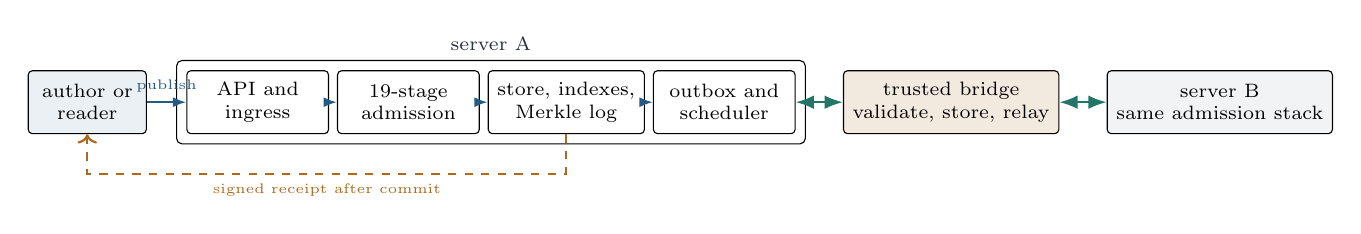
\begin{tikzpicture}[
  font=\scriptsize,
  box/.style={draw,rounded corners=1.5pt,minimum height=8mm,align=center,fill=white},
  core/.style={box,minimum width=18mm},
  edge/.style={-{Latex[length=1.7mm]},thick,jbblue},
  sync/.style={<->,>=Latex,thick,jbteal},
  group/.style={draw,rounded corners=2pt,inner sep=3.5pt}
]
  \node[box,minimum width=15mm,fill=jbblue!9] (client) {author or\\reader};

  \node[core,right=5mm of client] (ingA) {API and\\ingress};
  \node[core,right=1mm of ingA] (valA) {19-stage\\admission};
  \node[core,right=1mm of valA] (storeA) {store, indexes,\\Merkle log};
  \node[core,right=1mm of storeA] (outA) {outbox and\\scheduler};
  \node[group,fit=(ingA)(valA)(storeA)(outA),label={[font=\scriptsize,text=jbink]above:server A}] (srvA) {};

  \node[box,minimum width=19mm,fill=jbamber!14,right=6mm of outA] (bridge) {trusted bridge\\validate, store, relay};
  \node[box,minimum width=27mm,fill=jbgray,right=6mm of bridge] (srvB)
    {server B\\same admission stack};

  \draw[edge] (client) -- node[above,font=\tiny]{publish} (ingA);
  \draw[edge] (ingA) -- (valA);
  \draw[edge] (valA) -- (storeA);
  \draw[edge] (storeA) -- (outA);
  \draw[sync] (outA) -- (bridge);
  \draw[sync] (bridge) -- (srvB);
  \draw[->,dashed,jbamber,thick] (storeA.south) -- ++(0,-5mm)
    -| node[pos=.25,below,font=\tiny]{signed receipt after commit} (client.south);
\end{tikzpicture}
\caption{System architecture. Local and federated envelopes use the same admission and storage
path. Teal links carry caller-initiated synchronization over source-bound connections.}
\label{fig:architecture}
\end{figure*}

\subsection{Signed objects and admission}

An envelope contains a domain tag, object type, payload, public key, nonce, and expiry time. Its
identifier is the SHA-256 digest of specified canonical bytes. An Ed25519 signature covers the same
bytes \cite{bernstein2012ed25519}. Protobuf does not guarantee canonical serialization
\cite{protobufnotcanonical}. Our profile therefore fixes field order, requires minimal varints,
rejects unknown fields, and checks that decoding and re-encoding produces the original byte string.
The receiver does not normalize attacker-controlled bytes before signature verification.

Fig.~\ref{fig:pipeline} summarizes the admission path. Stages 1 to 12 check size, parsing,
canonicality, domain separation, identifier, signature, expiry, replay, and authorization without a
persistent write. Later stages apply origin pricing or peer quotas, commit the raw object and derived
indexes in one transaction, append its hash to a Merkle log, and enqueue federation only after the
commit. A database uniqueness rule makes exact retries idempotent.

\begin{figure}[t]
\centering
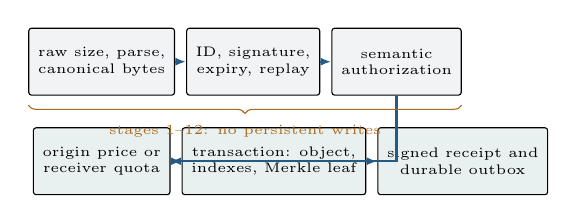
\begin{tikzpicture}[
  font=\tiny,
  pipe/.style={draw,rounded corners=1pt,minimum width=16.2mm,minimum height=8.5mm,
               align=center,fill=jbgray},
  wr/.style={pipe,fill=jbteal!10},
  arr/.style={-{Latex[length=1.35mm]},thick,jbblue},
  node distance=1.4mm
]
  \node[pipe] (raw) {raw size, parse,\\canonical bytes};
  \node[pipe,right=of raw] (crypto) {ID, signature,\\expiry, replay};
  \node[pipe,right=of crypto] (auth) {semantic\\authorization};
  \node[wr,below=4mm of raw] (quota) {origin price or\\receiver quota};
  \node[wr,right=of quota] (commit) {transaction: object,\\indexes, Merkle leaf};
  \node[wr,right=of commit] (after) {signed receipt and\\durable outbox};
  \draw[arr] (raw) -- (crypto);
  \draw[arr] (crypto) -- (auth);
  \draw[arr] (auth.south) |- (quota.east);
  \draw[arr] (quota) -- (commit);
  \draw[arr] (commit) -- (after);
  \draw[decorate,decoration={brace,amplitude=3pt,mirror},jbamber]
    ($(raw.south west)+(0,-1.2mm)$) -- ($(auth.south east)+(0,-1.2mm)$)
    node[midway,below=3.5pt,font=\tiny,text=jbamber]{stages 1--12: no persistent writes};
\end{tikzpicture}
\caption{Admission pipeline. State changes begin only after cheap byte and validity checks.}
\label{fig:pipeline}
\end{figure}

On acceptance, the server signs a receipt with the object identifier, leaf position, tree head, and
inclusion proof. This binds the acknowledgment to the submitted bytes. Peers also exchange signed
tree heads. A same-size, different-root pair is a clear conflict. A larger tree is marked pending
until a consistency proof is available. The current code therefore detects some log conflicts, but
does not yet prove append-only growth for every larger tree.

\subsection{Partition-aware federation}

Three caller-initiated remote procedure calls cover normal delivery and recovery.
\textsc{Deliver} sends a batch, \textsc{StreamActivities} resumes from a durable cursor, and
\textsc{Backfill} requests missing objects. A node with no public inbound endpoint can still send its
outbox and retrieve a peer's history over connections that it starts. This supports asymmetric
reachability such as carrier-grade network address translation, but it is not peer discovery. At
least one reachable address must already be known.

The scheduler drains independent per-peer queues with bounded concurrency, deadlines, backoff, and
idempotency keys. This prevents one unreachable peer from stopping work for a reachable peer. The
current deadline does not forcibly cancel the underlying library call, so stuck calls can still hold
resources longer than intended.

Fig.~\ref{fig:topology} shows the route-cut topology. Two ordinary nodes are placed in each simulated
island. The bridge has one address on each island network. After the ordinary inter-island route is
removed, both sides must explicitly trust the bridge. The bridge validates and stores every object,
limits volume per uplink pair and traffic class, and never sends an object back through the uplink on
which it arrived. Trust changes rate and priority policy, not object validity.

\begin{figure}[t]
\centering
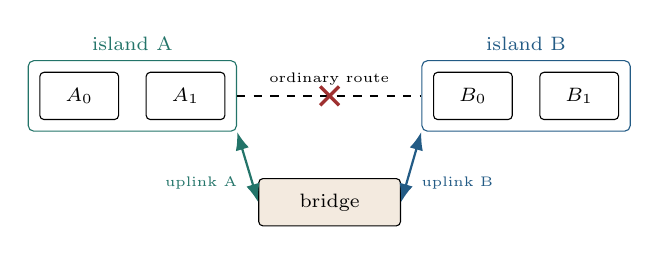
\begin{tikzpicture}[
  font=\scriptsize,
  node/.style={draw,rounded corners=1.5pt,minimum width=10mm,minimum height=6mm,fill=white},
  island/.style={draw,rounded corners=2pt,inner sep=4pt},
  link/.style={<->,>=Latex,thick,jbblue}
]
  \node[node] (a0) at (0,0) {$A_0$};
  \node[node] (a1) at (1.35,0) {$A_1$};
  \node[island,fit=(a0)(a1),draw=jbteal,
        label={[font=\scriptsize,text=jbteal]above:island A}] (ia) {};

  \node[node] (b0) at (5.0,0) {$B_0$};
  \node[node] (b1) at (6.35,0) {$B_1$};
  \node[island,fit=(b0)(b1),draw=jbblue,
        label={[font=\scriptsize,text=jbblue]above:island B}] (ib) {};

  \node[node,fill=jbamber!14,minimum width=18mm] (br) at (3.18,-1.35) {bridge};
  \draw[link,jbteal] (ia.south east) -- node[below left,font=\tiny]{uplink A} (br.west);
  \draw[link,jbblue] (br.east) -- node[below right,font=\tiny]{uplink B} (ib.south west);
  \draw[dashed,thick] (ia.east) -- node[above,font=\tiny]{ordinary route} (ib.west);
  \coordinate (cut) at (3.18,0);
  \draw[jbred,very thick] ($(cut)+(-0.12,-0.12)$) -- ($(cut)+(0.12,0.12)$);
  \draw[jbred,very thick] ($(cut)+(-0.12,0.12)$) -- ($(cut)+(0.12,-0.12)$);
\end{tikzpicture}
\caption{Four-node Docker topology. All containers run on one physical host. The bridge is an
application server, not an IP packet forwarder.}
\label{fig:topology}
\end{figure}

Four implementation rules protect replication. First, transport passes an opaque byte string to
ingress and cannot decode then re-encode it. Second, every peer, including a bridge, passes the full
validity checks. Third, database uniqueness handles duplicate delivery from a live stream and a
backfill. Fourth, fan-out excludes the origin peer. This avoids a redundant round trip even though
content deduplication would eventually stop a loop.

\section{Methodology}
\label{sec:method}

We evaluate five questions: whether independent encoders agree, whether objects cross an enforced
route cut, whether multi-hop delivery completes, whether malformed requests create storage writes,
and how the representation size compares with ActivityPub.

\textbf{Correctness tests:} A shared corpus contains 16 positive and adversarial byte vectors. The
TypeScript, Rust, and Python implementations run the corpus independently. Another 85 focused tests
cover ingress, outbox, federation, and simulated ISP behavior. These are regression tests, not an
independent security audit.

\textbf{Docker route-cut test:} Four application containers, four databases, and four caches use
three private Docker networks. The gate verifies source and destination addresses from kernel TCP
state, removes the ordinary inter-island path, confirms that direct probes fail, submits a dependent
certificate, community, and post, and polls for each exact content identifier. The gate contains 19
assertions for topology, source binding, relay, quota, and failover behavior. Reported time includes
the application's polling delay.

\textbf{Eight-node chain:} An in-process harness links eight servers in a line. It injects 200 valid
envelopes at hop 0 and records when each envelope reaches hop 7. This test isolates the federation
scheduler. It does not include container networking or external database services.

\textbf{Malformed-input run:} A client sends 3,000 oversized or non-canonical requests at
concurrency 16. We record completion rate, rejection class, entries into signature verification,
and persistent object count. The normal rate limiter remains enabled, so this is not a saturation
benchmark.

\textbf{Encoding comparison:} We collected 80 activities from two stock ActivityPub
implementations and retained their delivered JSON-LD contexts. We compared raw and gzipped activity
bytes with equivalent signed protobuf envelopes. Authored text was subtracted when computing
overhead. The test does not include HTTP framing, HTTP signatures, TLS records, follower fan-out, or
shared compression dictionaries. It measures representation size, not total protocol cost.

\section{Results}
\label{sec:results}

\subsection{Correctness and convergence}

All three implementations agreed on 16 of 16 canonical vectors and rejected every negative vector
as required. The focused tests also cover invalid signatures, non-canonical bytes, replay, missing
authorization dependencies, concurrent duplicate delivery, wrong receipt keys, invalid inclusion
proofs, stale tree heads, and same-size log conflicts. Sixteen vectors do not cover every protobuf
edge case, but they show that three independent implementations can follow the profile.

The Docker gate passed 19 of 19 assertions. After direct inter-island reachability was removed, the
destination saw the certificate after 0.5 seconds, the community after 1.2 seconds, and the post
after 2.1 seconds. The objects arrived in dependency order through the bridge. These values are one
controlled run, not a latency distribution.

All 200 envelopes in the eight-node chain reached hop 7. End-to-end median latency was 4.125 seconds
and the 99th percentile was 6.115 seconds. Fig.~\ref{fig:chain} shows the measured increase across
hops. The in-process setup has low contention and no wide-area delay, so the curve should not be used
to predict an Internet deployment.

\begin{figure}[t]
\centering
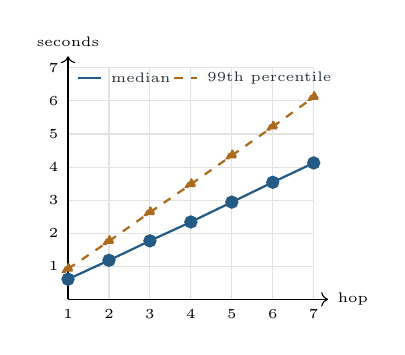
\begin{tikzpicture}[x=.52cm,y=.42cm,font=\scriptsize]
  \draw[gray!22,step=1] (1,0) grid (7,7);
  \draw[->] (1,0) -- (7.35,0) node[right,font=\tiny]{hop};
  \draw[->] (1,0) -- (1,7.35) node[above,font=\tiny]{seconds};
  \foreach \x in {1,...,7} \node[below,font=\tiny] at (\x,0) {\x};
  \foreach \y in {1,...,7} \node[left,font=\tiny] at (1,\y) {\y};
  \draw[jbblue,thick] plot[mark=*] coordinates
    {(1,.61)(2,1.18)(3,1.77)(4,2.34)(5,2.94)(6,3.54)(7,4.125)};
  \draw[jbamber,thick,dashed] plot[mark=triangle*] coordinates
    {(1,.92)(2,1.76)(3,2.63)(4,3.48)(5,4.35)(6,5.22)(7,6.115)};
  \draw[jbblue,thick] (1.25,6.7) -- (1.8,6.7) node[right,jbink,font=\tiny]{median};
  \draw[jbamber,thick,dashed] (3.6,6.7) -- (4.15,6.7)
    node[right,jbink,font=\tiny]{99th percentile};
\end{tikzpicture}
\caption{Eight-node in-process chain. All 200 envelopes reached hop 7.}
\label{fig:chain}
\end{figure}

\subsection{Admission and representation cost}

The malformed-input run completed at 730 requests per second and created zero object, index, log, or
outbox writes. However, 2,700 of 3,000 requests were stopped by rate limiting, and only about 9
percent entered signature verification. The supported conclusion is that the tested traffic did not
produce invalid storage writes. The experiment does not show resistance to distributed traffic,
valid signed floods, parsing pressure, or database contention.

Table~\ref{tab:tradeoff} reports the compression-aware ActivityPub comparison and the main costs of
the custom format. In the measured post, follow, and delete cases, gzipped ActivityPub used 4.4 to
6.9 times more representation bytes. This does not make the whole protocol better than ActivityPub.
The custom format cannot join the existing Fediverse, needs generated codecs and new operational
tools, and rejects unknown fields. Schema changes need a versioned domain or profile. ActivityPub's
JSON-LD model is easier to inspect with common web tools and is designed for extension. The custom
format instead chooses a small, explicit signed byte sequence.

\begin{table*}[t]
\caption{Measured representation size and design trade-offs against ActivityPub. The byte sample
contains 80 activities. Ratios use overhead after authored text is removed.}
\label{tab:tradeoff}
\centering
\scriptsize
\setlength{\tabcolsep}{4.2pt}
\begin{tabularx}{\textwidth}{>{\bfseries}p{21mm}p{51mm}p{51mm}X}
\toprule
Dimension & This work & ActivityPub comparison & Cost or boundary \\
\midrule
Measured bytes & Signed envelopes: post 206, follow 142, delete 250 & Gzipped JSON-LD: post 1,074,
follow 786, delete 1,400; observed overhead ratio 4.4--6.9$\times$ & Representation only; HTTP, TLS,
fan-out, and shared dictionaries are excluded \\
Interoperability & Custom protobuf domains and RPCs & Standard actor, object, and inbox model & No
direct Fediverse compatibility or existing application ecosystem \\
Evolution & Unknown fields rejected; versioned profiles required & Flexible JSON-LD vocabulary and
extensions & Harder rolling upgrades and more cross-language test work \\
Operations & Generated codec and canonical-byte tools required & Text can be inspected with common
web tools & Higher debugging and tooling burden for operators \\
Integrity profile & One exact object byte string, content ID, author signature, and receipt &
Authentication choices depend on the deployment profile & Clear byte identity, but a new security
profile must be maintained and audited \\
\bottomrule
\end{tabularx}
\end{table*}

\section{Discussion and Limitations}
\label{sec:limits}

\textbf{Docker test boundary:} Docker gives repeatable private layer-2 segments and lets the gate
remove the only configured path between them. It does not reproduce an ISP. All containers share one
host, kernel, clock, CPU, and storage system. Docker's virtual bridges, fixed container addresses,
and local name resolution are simpler than physical routers, Border Gateway Protocol changes,
carrier-grade network address translation, real DNS failure, variable maximum transmission units,
and radio access. The dual-homed bridge is also easy to attach to both Docker networks. A real bridge
would need separate links, routing policy, credentials, power, and operators. Therefore, the route-cut
test shows software and routing state changes, not geographic latency, independent failure domains,
or real ISP behavior.

\textbf{Access and subscriber isolation:} The design assumes that servers inside an island can reach
each other or a shared bridge. Wi-Fi access point (AP) client isolation, or ISP subscriber and IP
isolation, can block direct traffic between customers even when each customer can still reach the
provider gateway. If this isolation is active on every surviving path, nodes cannot dial or bridge
to one another. Full federation then fails, and only separate local service remains. The current
prototype has no non-IP fallback for this case.

\textbf{Network adversary:} A network operator can identify stable endpoints, block IP addresses or
server name indication values, fingerprint remote procedure call traffic, analyze timing, isolate a
node, or coerce a bridge. Source-address binding chooses an uplink but does not hide it. A total
power, radio, and packet outage leaves no path. Multiple independent bridges, endpoint rotation, and
pluggable transports may reduce some risks, but they were not evaluated.

\textbf{System and application limits:} Signatures authenticate keys, not truth or safety. A valid
key can submit abuse or a costly flood. A malicious origin can omit its own admission price, so the
receiver still needs quotas. Key theft, metadata leakage, moderation, revocation recovery, storage
exhaustion, and coordinated Sybil behavior remain open. The transport deadline does not cancel the
underlying call. Log consistency proofs for growing trees are not implemented. A receipt proves
acknowledged acceptance, not universal availability or prompt forwarding.

\textbf{Evaluation limits:} The route-cut result comes from one preserved run. The chain uses eight
in-process nodes, and the encoding sample has 80 ActivityPub activities from two implementations.
There are no multi-host, wide-area, multi-day, or real-shutdown trials. Host load, repeated-run
distributions, and confidence intervals were not preserved. Comparisons with phone encounter and
voice-channel systems use different workloads and should not be read as a ranking.

\textbf{Ethics:} The tests used synthetic content and isolated private networks. A real deployment
could expose bridge operators and users to legal or physical risk. A visible relay should not be
deployed in a hostile setting without local threat analysis, informed consent, data minimization,
and legal and community review.

\section{Conclusion}

This work shows that server federation can continue across a simulated route cut when some IP paths
survive. Canonical signed objects, one admission path, caller-initiated recovery, and a trusted
validating bridge carried a dependent post across two Docker network islands. Cross-language tests
and an eight-node chain provide additional evidence. The smaller representation comes with clear
costs: it loses ActivityPub interoperability, easy extension, and mature tooling. The most important
next steps are multi-host and wide-area experiments, log consistency proofs, cancellation-aware
transport, valid-traffic stress tests, several independent bridges, and a non-IP fallback for access
or subscriber isolation and total blackouts.

\IEEEtriggeratref{18}
\bibliographystyle{IEEEtran}
\bibliography{../../paper/references}

\end{document}
